\documentclass[12pt]{scrarticle}

\usepackage[utf8]{inputenc}
\usepackage{graphicx}
\usepackage{listings}
\usepackage[colorlinks=true, citecolor=blue]{hyperref}
\usepackage{amsmath}
\usepackage{lipsum}
\usepackage{caption}
\usepackage{subcaption}
\usepackage{float}
\usepackage[backend=biber,
            style=apa,
            citestyle=apa]{biblatex}
\addbibresource{Running-Example/Workshop-Latex.bib}

\title{A running Example of Latex}
\author{Daniel Anthes \and Moritz Nipshagen}
\date{} % defaults to today

\begin{document}

\maketitle

\begin{abstract}
    \lipsum[3]
\end{abstract}

\section{I am a section}

\lipsum[1]

\subsection{I am a subsection}

\lipsum[2]

\section{Math}

Here is an inline formula: $e = mc^2$.

One more, but now on a separate line:

$$
\mathcal{N}(x|\mu, \sigma) = \frac{1}{\sigma \sqrt{2\pi}}\exp \left({\frac{(x - \mu)^2}{2\sigma^2}}\right)
$$

Now with multiple aligned formulas:

\begin{eqnarray}
\dot{x_1} &=& -x_2 + x_{2}^3\\
\dot{x_2} &=& -x_1 + x_{1}^3
\end{eqnarray}

Notice that \textit{eqnarray} numbers the formulas. Add a star to disable numbering:


\begin{eqnarray*}
\dot{x_1} &=& -x_2 + x_{2}^3\\
\dot{x_2} &=& -x_1 + x_{1}^3
\end{eqnarray*}

\section{Images}

\begin{figure}[h!]
    \centering
    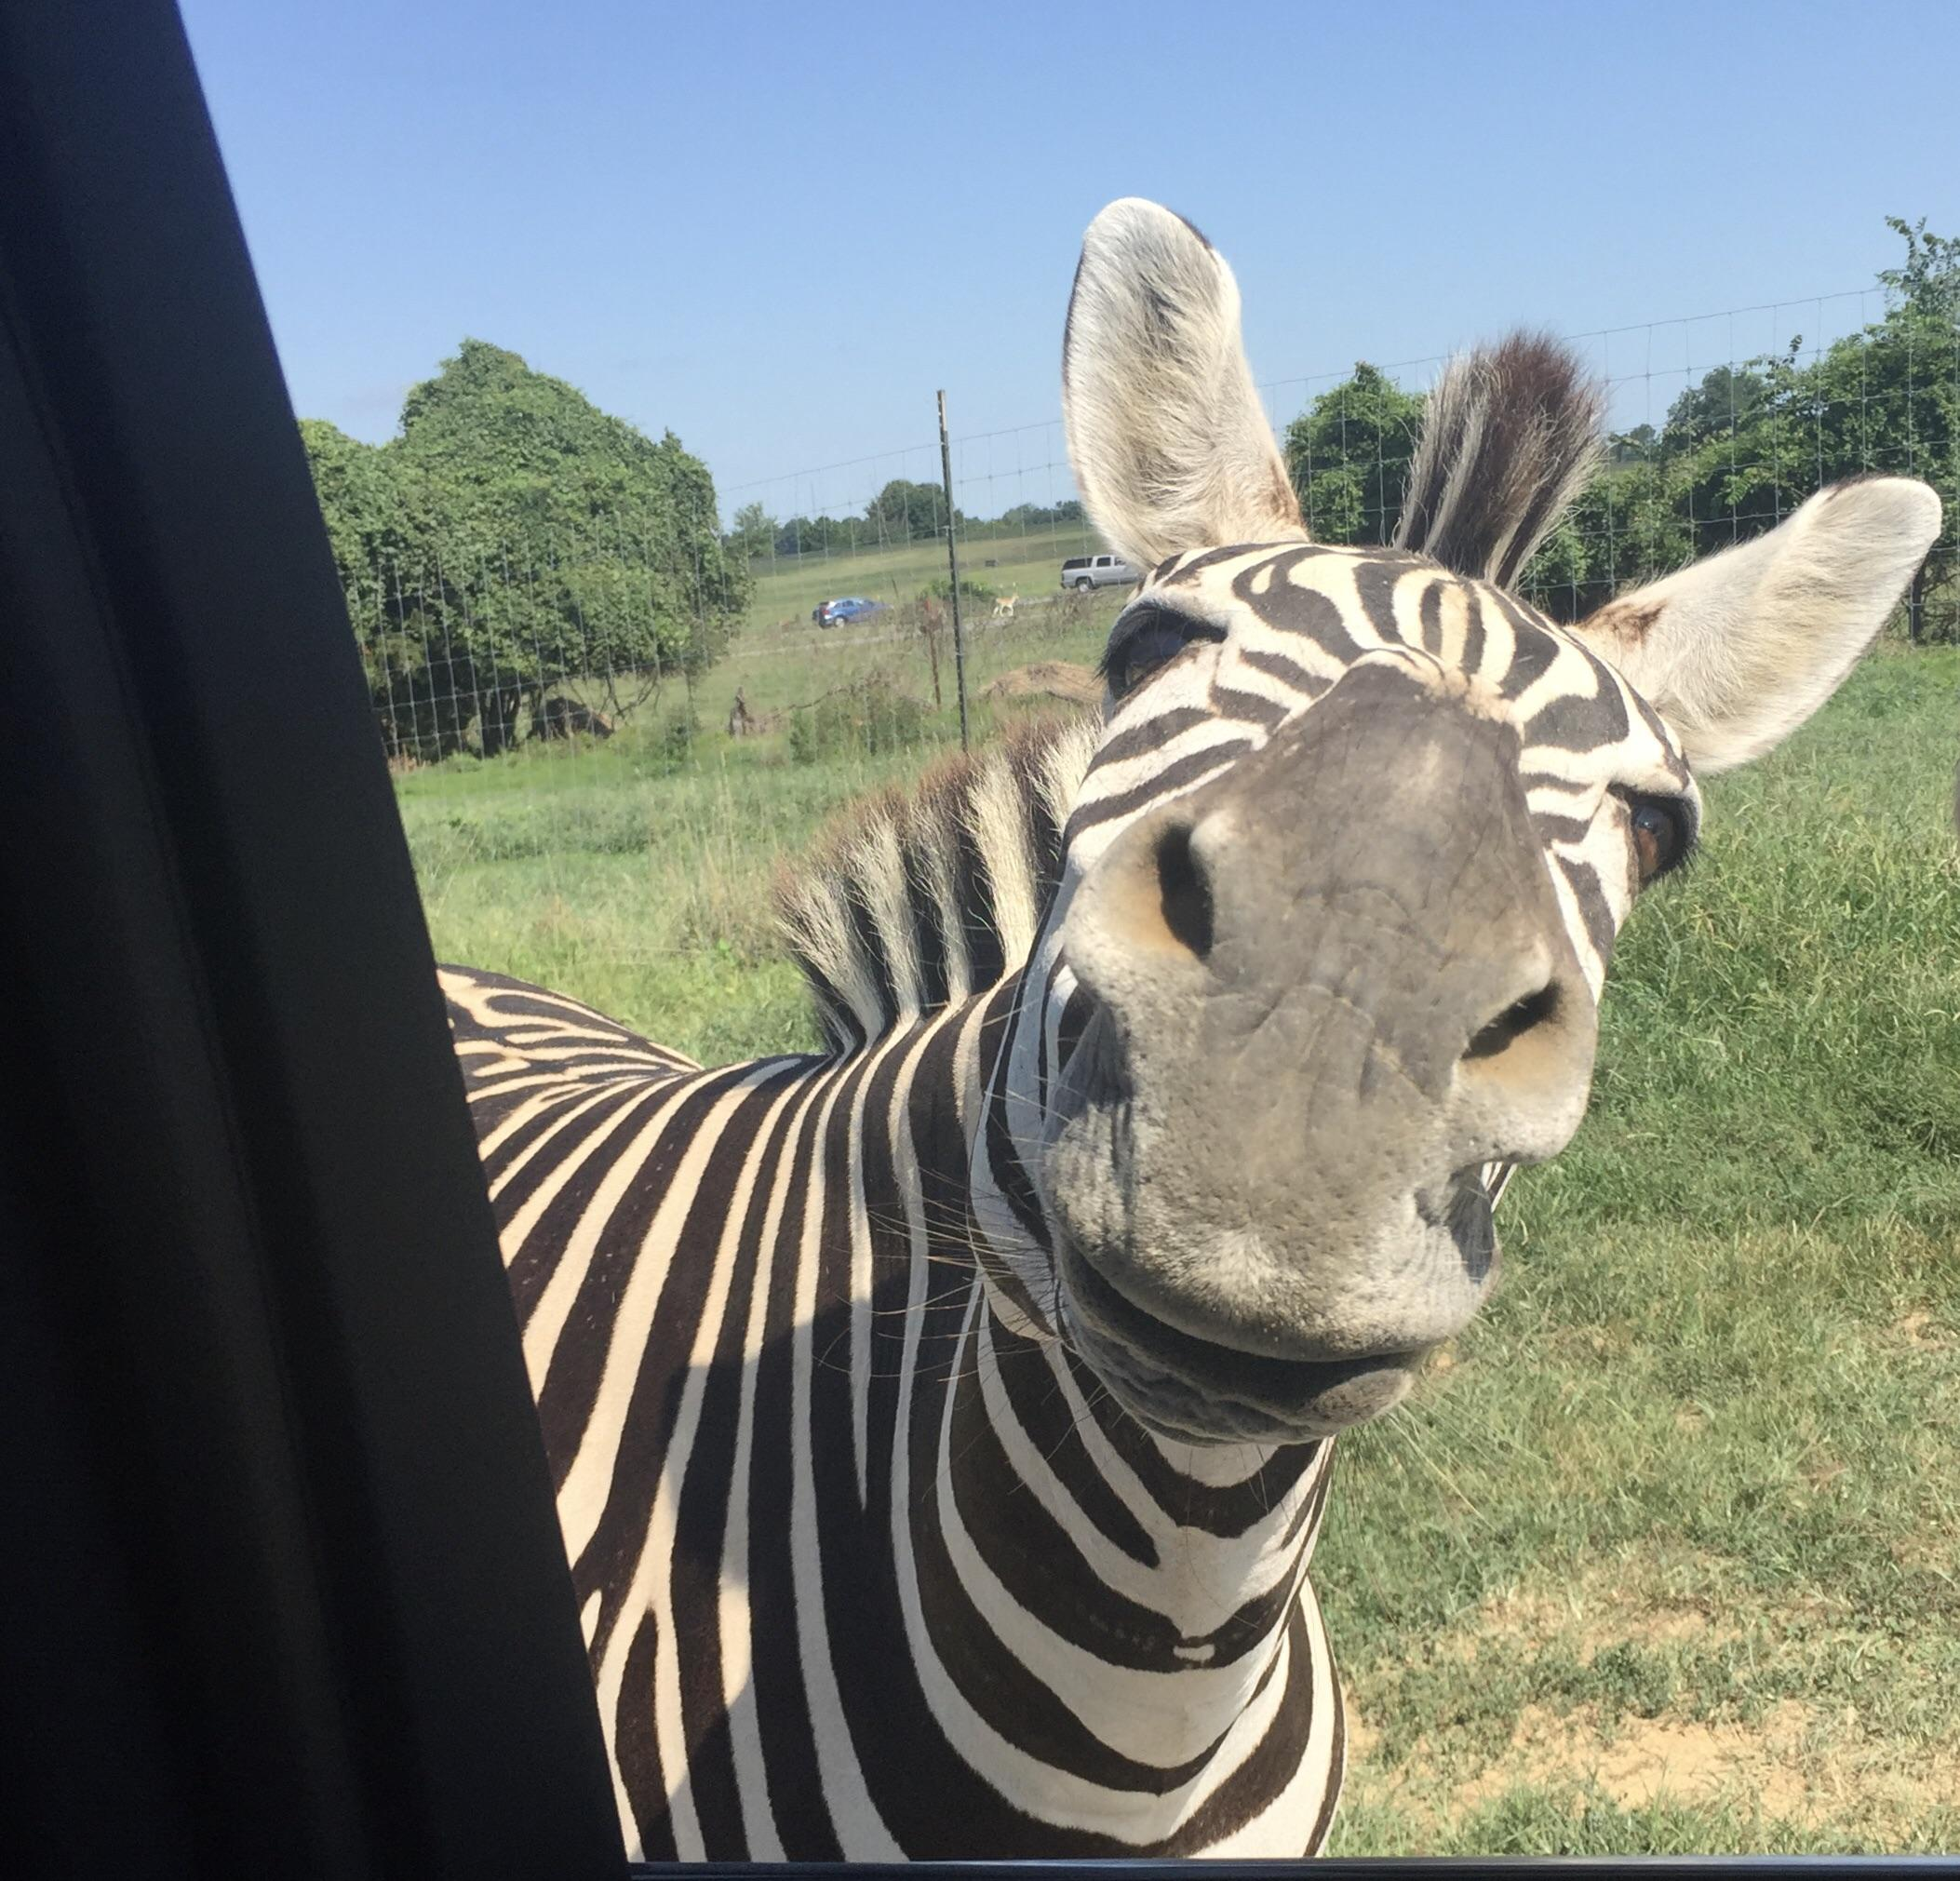
\includegraphics[width=.3\linewidth]{Running-Example/zebra.jpeg}
    \caption{Zebra.}
    \label{fig:examplefig}
\end{figure}

We can also have multiple images in a figure:

\begin{figure}[H]
    \centering
    \begin{subfigure}{0.49\textwidth}
        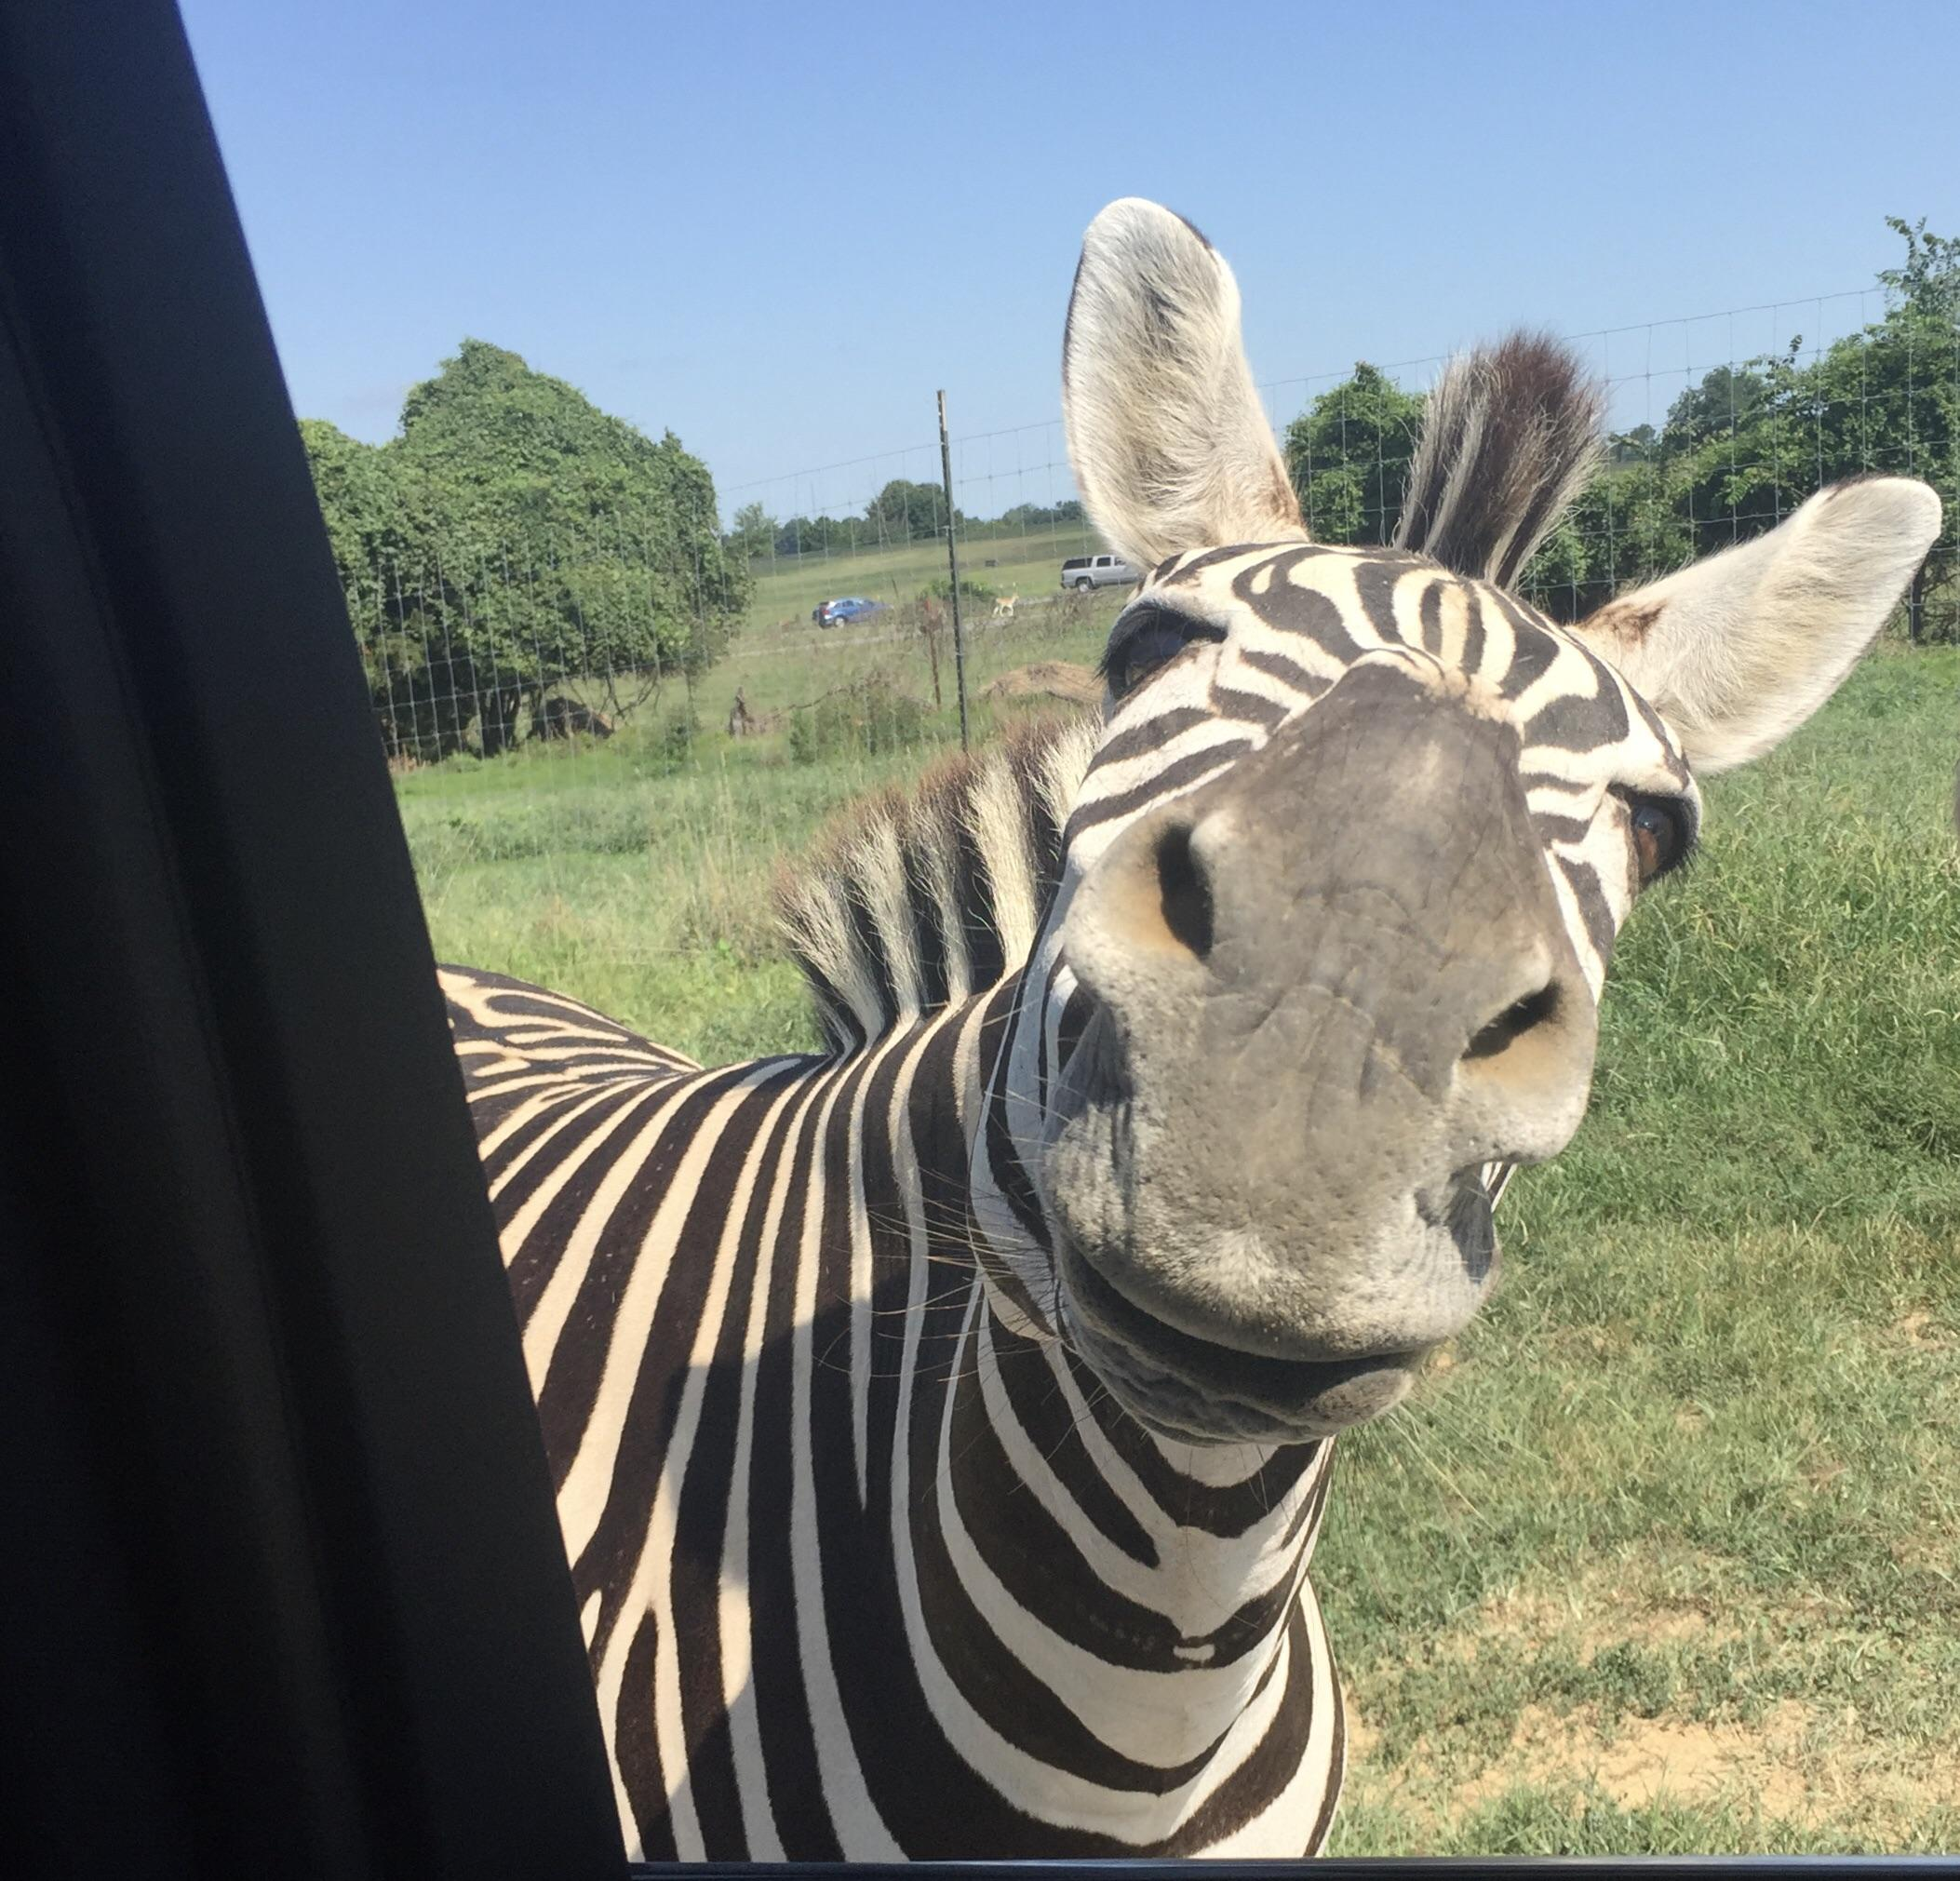
\includegraphics[width=0.9\linewidth]{Running-Example/zebra.jpeg}
        \caption{Zebra.}
    \end{subfigure}
    \begin{subfigure}{0.49\textwidth}
        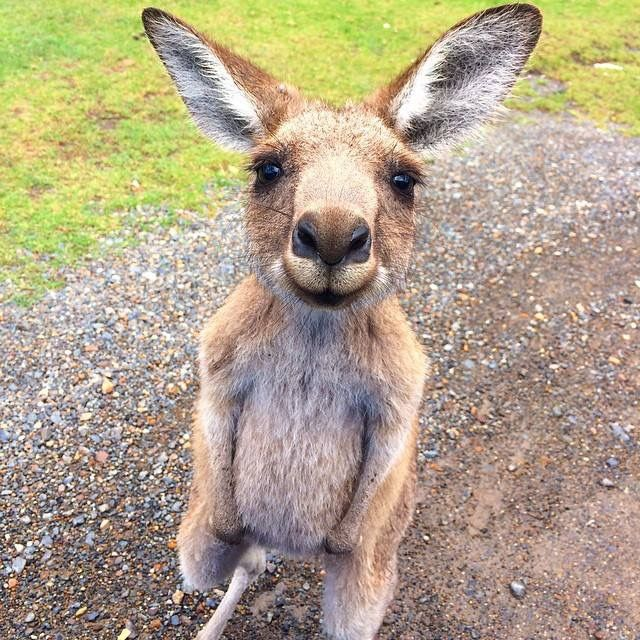
\includegraphics[width=0.9\linewidth]{Running-Example/kangaroo.jpeg}
        \caption{Kangaroo.}
    \end{subfigure}
    \caption{Animals.}
    \label{fig:animals}
\end{figure}

This document contains a lot of figures and not a lot of text. When this happens latex can sometimes have trouble placing the figures and tables in a nice way. We use the \textit{float} package to tell Latex to put figures exactly where we want them. (with the optional argument \textit{H})

\section{Tables}

\begin{table}[H]
    \centering
    \begin{tabular}{|l||c|c|c|}
    \hline 
    Animal & Is Zebra & Is Pet & Legs\\
    \hline\hline
    Dog         & No    & Yes   & 4\\
    Cat         & No    & Yes   & 4\\
    Zebra       & Yes   & No    & 4\\
    Kangaroo    & No    & No    & 2\\
    \hline
    \end{tabular}
    \caption{Animal Facts}
    \label{tab:my_label}
\end{table}

\section{Links, References and Footnotes}

Here is a link: \url{https://dondrite.ruhosting.nl}

And one that has an alternative text: \href{https://www.youtube.com/watch?v=dQw4w9WgXcQ}{A clickable link!}

You can also refer to elements with a label in your document: (\ref{fig:examplefig})

Footnotes are also possible, and clickable\footnote{If you are using the \textit{hyperref} package}

\section{Styling}

You can have \textit{italic} and \textbf{bold} text, \texttt{monospaced} and \textsc{small caps}. Text can also be {\large{large}}, {\Large{larger}}, {\huge huge} and {\Huge really Huge} or {\small{small}} and even {\tiny tiny}.

\begin{center}
    you can center your text as well
\end{center}

And {\color{blue}colors} {\color{red} are} {\color{cyan} also} possible.

Notice that commands such as \textit{color} or \textit{small} affect the rest of the current environment. You can set a "scope" by surrounding the text to be affected by the command with curly braces.

\section{References}

\subsection{How to get your references into format}
Latex uses \texttt{.bib} files that are structured in a specific manner. Each entry in that document is prefaced by an \@\textit{category} followed by curly braces \{ that contain tags with information like, author, date, publication \}. You don't have to memorise this though.
\subsubsection{Manual Labour: Copy \& Pasting}
Most of your favourite platforms provide bib(la)tex style citations to copy and paste into your file.
\begin{figure}[H]
    \centering
    \begin{subfigure}{0.49\textwidth}
        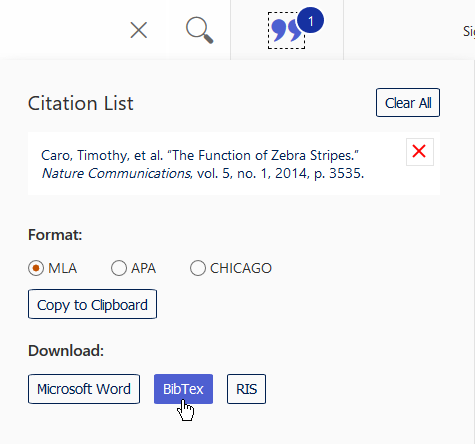
\includegraphics[width=0.9\linewidth]{Running-Example/academic_microsoft.png}
        \caption{Exporting citations from \url{academic.microsoft.com}}
    \end{subfigure}
    \begin{subfigure}{0.49\textwidth}
        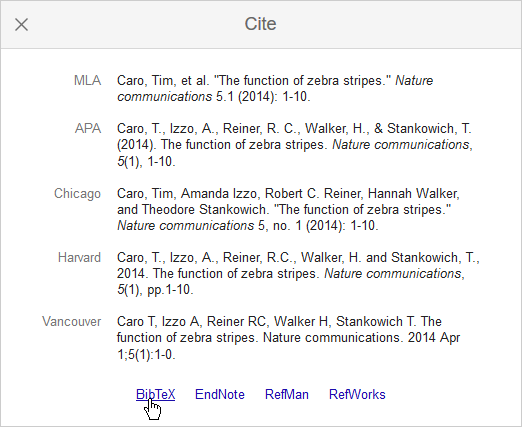
\includegraphics[width=0.9\linewidth]{Running-Example/scholar_google.png}
        \caption{Exporting citations from \url{scholar.google.com}}
    \end{subfigure}
    \caption{Options to download in bibtex format from common paper aggregators.}
    \label{fig:citations}
\end{figure}
You can then upload / paste the contents to your reference \texttt{.bib} file, load them with biblatex and use them in your document. Once  they are there, you don't have to manually change the style, reference or make sure that everything you cited is your reference list. 
However, if you don't want the manual download / pasting, pretty much all sources for references supply \texttt{.ris} files, which you can import in a reference manager.

\subsubsection{The Glory of Reference Managers}
If you are not already, we firmly urge you to consider using one (no matter if you use latex or not)\footnote{We personally like to use \href{https://www.zotero.org/}{Zotero}. It's free, has a bunch of functions and plugins and supports latex, word and more.}. Most managers have an internal search which you can use to add references to your database, and if they don't find it you can use the \texttt{.ris} file supplied by the websites to import it. Once you have your collection ready, you can export all the references to a \texttt{.bib} file (see figure \ref{fig:zotero}) and then use that for your overleaf document. A lot less hassle, you don't accidentally delete or overwrite something and you can tag and sort and file your references for different projects without needing to track a lot of files.

\begin{figure}[h]
    \centering
    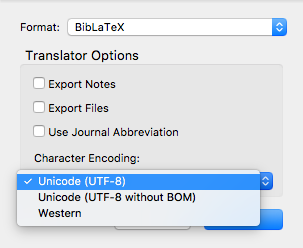
\includegraphics[width=.4\textwidth]{Running-Example/zotero_export.png}
    \caption{The zotero export window}
    \label{fig:zotero}
\end{figure}

\subsection{Talk to the Manager: Biblatex}

The package that handles all of the nice reference commands and organisation is called \textbf{biblatex}. You import it like any other package: \texttt{\textbackslash usepackage\{biblatex\}}. When importing you can give it a bunch of options, like the citation style to use, like this: \texttt{\textbackslash usepackage[backend=biber, style=apa, citestyle=apa]\{biblatex\}}. You basically always want to default to using the biber backend, unless you have a reason not to. The \texttt{style} option is the style for the bibliography and the \texttt{citestyle} option is for inline citations.\\
Once you imported biblatex, you can tell it where to find your references with the \texttt{\textbackslash addbibresource} command, which in our case looks like this:\\
\texttt{\textbackslash addbibresource\{Running-Example/Workshop-Latex.bib\}}.

\subsubsection{Citation Styles and Bibliography}

Citations in your text are added with \textit{cite} (\cite{caroFunctionZebraStripes2014}). $\leftarrow$ to generate this citation we used\\
\texttt{\textbackslash cite\{caroFunctionZebraStripes2014\}}. The identifiers often look like \textit{authorTitleYear}, but can be set by yourself as well.

To generate your bibliography at the end of the document add \textit{printbibliography}

\printbibliography

\end{document}